% AUTHOR: Agostino De Marco, agostino.demarco@unina.it
% LaTeX STARTING DECLARATION
\documentclass[12pt,twoside]{book}
\usepackage{_my_document_style}
\usepackage{pdfpages}
% BEGIN DOCUMENT

\begin{document}

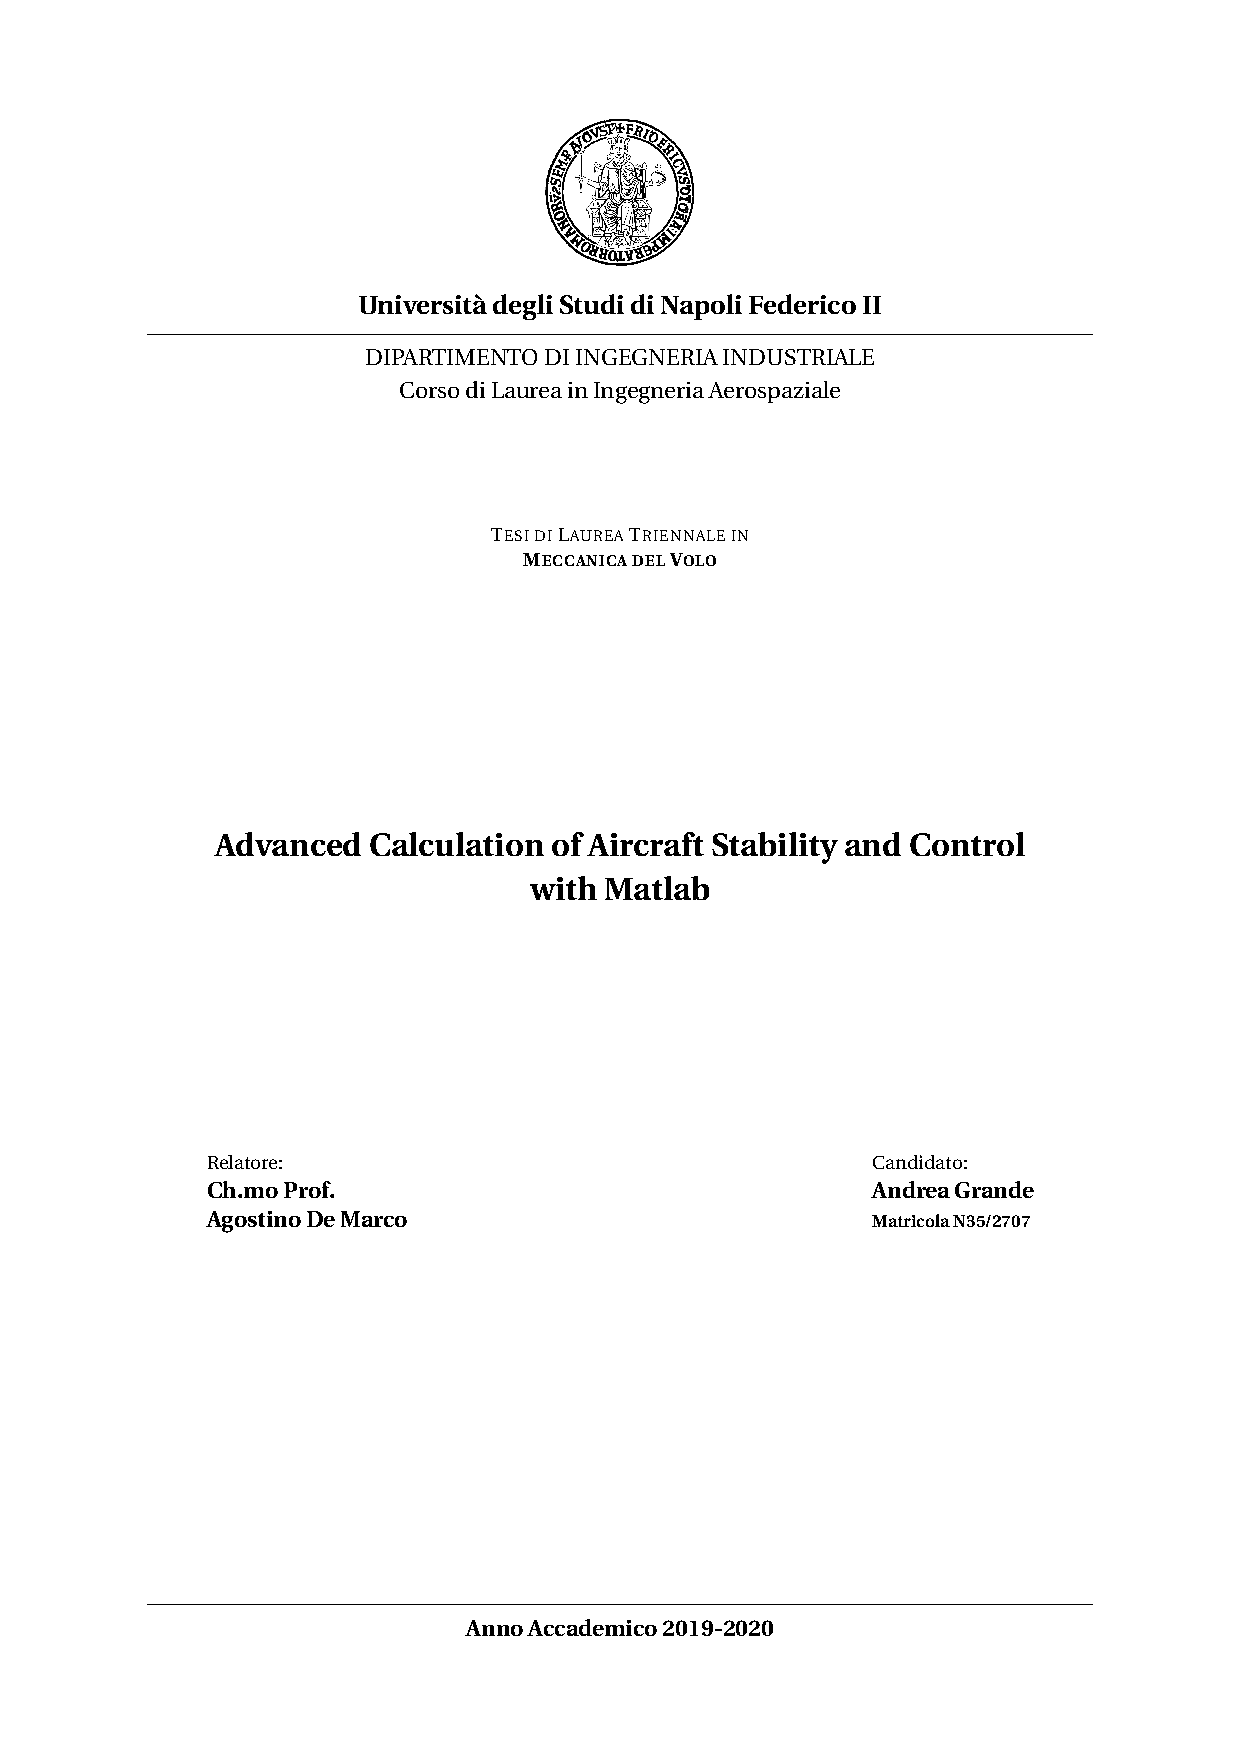
\includepdf[pages={1}]{frontespizio.pdf}
%
\newpage
%
\import{}{backcover_page}
%
\newpage
%
\import{}{copyright_page}
%
\cleardoublepage
%
% minitoc stuff -----------
%\mtcsetpagenumbers{*}{off}
\dominitoc \dominilof \dominilot
%\faketableofcontents
\tableofcontents
%\fakelistoffigures \fakelistoftables
\listoffigures
%
%
\chapter*{Introduction}
\addcontentsline{toc}{chapter}{Introduction}
\import{Introduction/}{introduction_page}
% -------------- minitoc stuff
%
%
\mainmatter
%
%?[ADJUST-HERE] PLACE THIS AS NEEDED
\renewcommand{\thechapter}{\arabic{chapter}}
%
%
\opt{final}{% <===
  \import{Chapter_1/}{chapter_1}
  \import{Chapter_2/}{chapter_2}
  \import{Chapter_3/}{chapter_3} \import{Chapter_4/}{chapter_4}
}

%% reset the material handled by package background
\makeatletter
\renewcommand{\bg@material}{}%
\makeatother

% -------   A P P E N D I C E S
% some configuration commands by package appendix
% some configuration commands by package appendix
\clearpage \phantomsection
\renewcommand{\chaptername}{Appendix}
\renewcommand{\appendixtocname}{Appendix}
\renewcommand{\appendixpagename}{Appendix}
\appendixpage
\noappendicestocpagenum
\addappheadtotoc
\pagestyle{myAppendixPageStyle}

%Here we include the appendix material of the book

\begin{appendices}% needs package appendix

\import{appendices/}{appendices}

\end{appendices}
%Here we include the appendix material of the book

% ---  B I B L I O G R A P H Y
\clearpage \phantomsection
\addcontentsline{toc}{chapter}{Bibliography}
\pagestyle{myBibliographyPageStyle}
\nocite{*}  
%\printbibheading[title={Bibliography}]
\printbibliography[heading=myBibliography]% needs biblatex
 
% ---  P R I N T   G L O S S A R Y   and   A C R O N Y M S
% add all the entries to the glossaries without referencing each one explicitly
\glsaddall
% 
\glossarystyle{list}%    can choose other style for displaying glossaries
% styles -->   list, listdotted, long, longragged, super, tree
%
%\printglossaries
%%%
%%  other possible uses:


% \markboth{}{}
% \clearpage
% \pagestyle{myGlossaryPageStyle}
%  \printglossary[type=main]% the default glossary is printed

\markboth{}{}
\clearpage
\pagestyle{myListOfSymbolsPageStyle}
\printglossary[type=symbols]

% ---   I N D E X
% \markboth{}{}
% \cleardoublepage
% \pagestyle{myIndexPageStyle}
%
% \markboth{}{}
% \clearpage
% \pagestyle{myAcronymsPageStyle}
% \printglossary[type=\acronymtype]
% %
% \indexnote{%
% In the index we have many voices, of various types. The page number on the right
% reveals where those terms appear in the book.%{\parfillskip=0pt\par}

% \medskip\noindent
% \blindtext% this is just some dummy text

% \medskip
% {\color{red}
% The index---and index entries---should be the very last thing to work at when writing a book!
% So, do not worry about what you see below. These items are going to change many times before
% the final version of the document is released.}
% }% end-of-indexnote

% \phantomsection
% \printindex
%
%\markboth{}{}
%\cleardoublepage
%
% ---  T O   D O   L I S T
%
%\listoftodos[List of TO-DOs and comments]
%
% ------------------------------------------------------ 
\chapter*{Acknowledgments}
\addcontentsline{toc}{chapter}{Acknowledgments}
\import{Acknowledgments/}{acknowledgments}
%
\end{document}

%% Notes
% https://www.latex4technics.com/